\chapter{Problem Statement}
\label{cha:multiObjectiveOptimization}



%---------------------------------------------------------------------------

\section{Multi-Objective Optimization}
\label{sec:strukturaDokumentu}

Multi-objective optimization is used to solve problems involving more than one objective function.
Such problems are often encountered in real world so efficient methods of solving them have wide applications.
(\cite{Deb:2001:MOU:559152})

%TODO: MCDM, MOOP

Each conflicting objective corresponds to a different optimal solution.  
It is obvious that solution that is optimal with respect to one objective requires a compromise in other objectives.
Because of this reason, in order to compare two solutions we have to introduce ordering relation.

Pareto front is the set of choices that are Pareto efficient. 

%---------------------------------------------------------------------------

\section{Modern Portfolio Theory}

%---------------------------------------------------------------------------

\section{Capital Asset Pricing Model}

%\cite{CAPM}

Capital Asset Pricing Model was developed in 1960s by Sharpe (\cite{CAPM-Sharpe}) and Lintner.
It tries to find the relationship between the price of a single asset and its risk.
Answering the question of how to calculate a risk as well as return of any asset being a part of portfolio is of paramount importance to each investor.

The Sharpe capital asset pricing model is based on the following assumptions \cite{CAPM}:

\begin{itemize}
  \item all investors are risk aversing
  \item all investors have the same information about the market
  \item capital markets are perfect - no transaction costs, no tax, all assets are infinitely divisible
  \item all investors view the expected returns and standard deviations of return provided by different portfolios in the same way
\end{itemize}
 
Lets assume that investor portfolio contains $N$ assets, then according to Capital Asset Pricing expected return of asset $i$ is \cite{CAPM}: 

\begin{equation}
\label{first_eq}
 E(R_{i})  = R_{f} + \frac{ [E(R_{m}) - R_{f}]} {(\sigma^2(R_{m}))} cov(R_{i}, R_{m})
\end{equation} 

\begin{description}
  \item [$E(R_{i})$]
    expected return of asset $i$
  \item [$R_{f}$]
    risk-free rate of interest (e.g. government bonds)
  \item [$E(R_{m})$]
    expected return of the market
  \item [$\sigma^2(R_{m})$]
    variance of the market return
  \item [$cov(R_{i}, R_{m})$]
    covariance between market return and asset $i$ return
\end{description}

While the risk associated with entire portfolio is equal to:

\begin{equation}
\label{sec_eq}
 \sigma_{p}  = \sqrt{\sum_{i} \sum_{j} w_{i}w_{j} \sigma_{i} \sigma_{j} \rho_{ij}}
\end{equation} 

\begin{description}
  \item [$\sigma_{p}$]
    portfolio risk
  \item [$w_{i}$]
    weighting of component asset i
  \item [$w_{j}$]
    weighting of component asset j
  \item [$\sigma_{i}$]
    standard deviation of asset $i$
  \item [$\sigma_{j}$]
    standard deviation of asset $j$
  \item [$\rho_{ij}$]
    correlation coefficient between the returns on assets i and j
\end{description}
 


%---------------------------------------------------------------------------


\section{Trend following}
\label{sec:trendFollowing}

\subsection{Trend following fundamentals}
\label{sec:trend_following_fundamentals}

The concept of price as the trading cue lays the foundations for trend following. 
Contrary to other trading strategies based on fundamental analysis (which use factors like: overall state of the economy, interest rates, production, etc. to predict stock price)
trend following use only price as the key trading variable. 

Trend following basically does not try to predict when the trend will occur. 
It simply analyses stock prices and decides whether the current situation is suitable for buying or selling a specific stock.
Market breakouts are a great buying opportunities, when you recognize that you are wrong you exit immediately in order to cut losses.
Set of predefined rules decides  whether to take any action (they should recognize when the trend starts as well as when to exit) so the entire process can be easily automated.
Such rules are quite simple but disciplined execution of them could lead to acheiving spectacular returns year after year.
It is all about cutting the losses and letting the profits run.
Many leading hedge funds successfully use strategies based on trend following to manage their portfolios. (\cite{Trend01})  

\newpage
\begin{figure}[ht]
  \begin{center}
    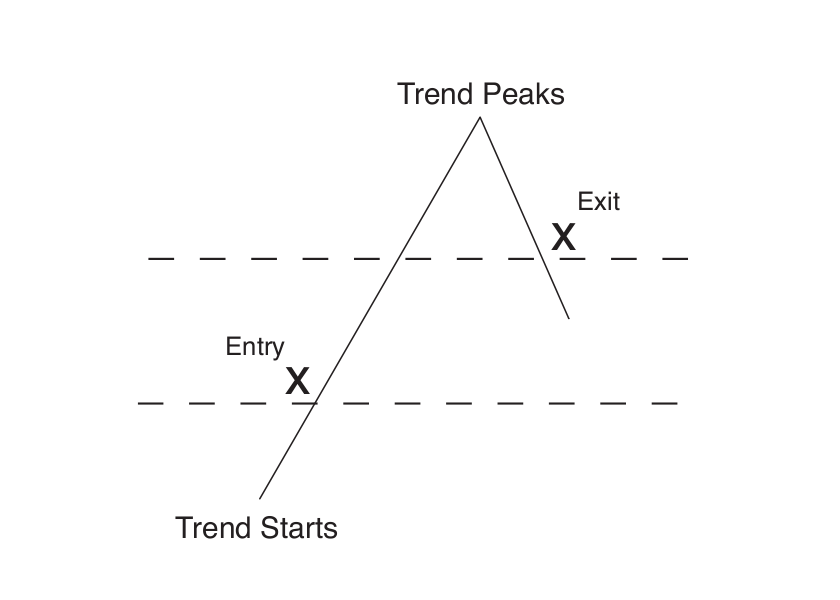
\includegraphics[scale=.4]{trend_following.png}
  \end{center}
  \caption{Simple example of how trend following works in practise}
\end{figure}

Another advantage of this investing method is the fact that investor does not have to know much about what is being traded (it could be stocks, oil, gold, etc.).
Normally, people tend to gather some information about the company they are willing to invest in. 
They analyse its market situation, competitors, financial performance, etc. which is time consuming, especially for someone who is not a professional trader.
With trend following we just have to to focus on elaborating trading rules that should reflect our trading strategy.
After that we can automate the decision making process by designing and implementing our own trading system.   


\subsection{Designing trading system based on trend following} 

Following \cite{Trend01}, the core of each trading system based on trend following strategy is a set of rules governing each buy/sell decision.
More specifically we have to devise rules to answer the following questions:

\begin{itemize}
  \item how much money are we willing to put on a single trade
  \item when to exit (what kind of losses are acceptable)
  \item when to enter (when the trend has started) 
  \item what markets are we interested in and how to split money between them (we would like to have a diverse portfolio (stocks, gold, etc.))
\end{itemize}

These rules should reflect our investing style.

In \ref{trend_following_impl} a system based on trend following strategy is presented in more details.

%---------------------------------------------------------------------------

\section{Genetic Algorithms}
\label{sec:genAlgorithms}

Many computational problems require searching through a huge number of possibilities for solutions.
Such search problems can often benefit from an effective use of parallelism, in which many different possibilities are explored simultaneously in an efficient way. 
It turns out that the process of biological evolution could provide the inspiration for addressing these problems.
(\cite{Mitchell01})

The genetic algorithm (GA) is an optimization and search technique based on the principles of genetics and natural selection.
A GA allows a population composed of many individuals to evolve under specified selection rules to a state that maximizes the “fitness” (i.e., minimizes the cost function).
The method was developed by John Holland (1975) over the course of the 1960s and 1970s.(\cite{Haupt:2004:PGA:1007746})



\subsection{Elements of genetic algorithms}

Almost all genetic algorithms have some elements in common \cite{Mitchell01}:
\begin{itemize}
  \item populations of chromosomes
  \item selection according to fitness
  \item crossover to produce new offspring
  \item random mutation of new offspring
  \item fitness function
\end{itemize}

\begin{figure}[ht]
  \begin{center}
    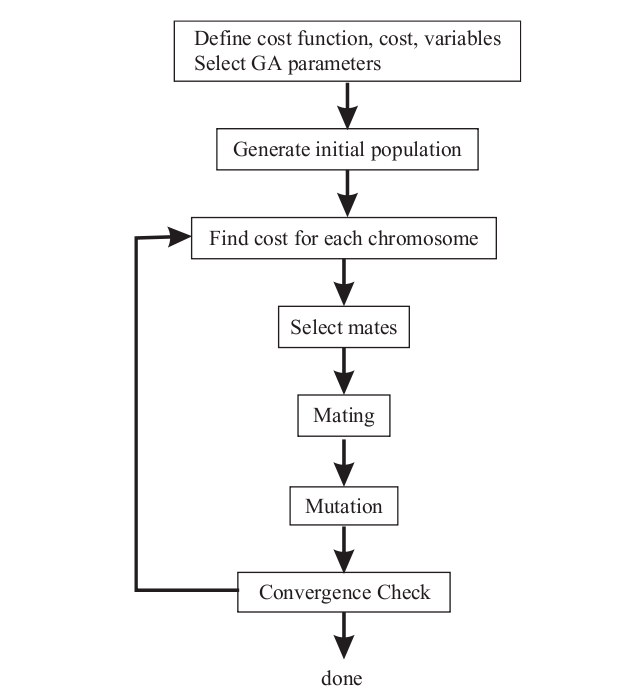
\includegraphics[scale=.4]{GA_flow.png}
  \end{center}
  \caption{GA flow chart \cite{Haupt:2004:PGA:1007746}}
\end{figure}

The GA processes populations of chromosomes, succesively replacing one such population with another (by using GA operators: mutation, selection, crossover, etc.). 
Each chromosome contains potential solution to problem (e.g. represented as binary string). 
Fitness functions are used to assess how well specific chromosome solves the problem.
The better fitting chromosomes are more likely to be involved in reproduction process.
That mimics the biological process of evolution - fitness of an organism is obtained by means of simple variation (mutation, recombination, etc.) and natural selection
thus propagating genetic material to future generations.
These rules seems to be simple but they are in fact responsible for extraordinary variety and complexity of the biosphere.
\cite{Mitchell01} 
 
According to \cite{Mitchell01} , GAs work by discovering, emphasizing, and recombining good "building blocks" of solutions in a highly parallel fashion.
The idea here is that good solutions tend to be made up of good building blocks-combinations of bit values that confer higher fitness on the strings in which they are present.

 

\subsection{Genetic algorithms operators}

Following \cite{Mitchell01} - the simplest form of genetic algorithm involves three types of operators: selection, crossover and mutation. 

\begin{description}

\item[selection]
  This operator selects chromosomes in the population for reproduction.
  The fitter the chromosome, the more times it is likely to be selected to reproduce.
  
\item[crossover]
  This operator randomly chooses a locus and exchanges the subsequences before and after that locus between two chromosomes to create two offspring.
  For example, the strings 10000100 and 11111111 could be crossed over after the third locus in each to produce the two offspring 10011111 and 11100100.
  The crossover operator roughly mimics biological recombination between two single-chromosome organisms.

\item[mutation]
  This operator randomly flips some of the bits in a chromosome.
  For example, the string 00000100 might be mutated in its second position to yield 01000100.
  Mutation can occur at each bit position in a string with some probability, usually very small (e.g., 0.001).


\end{description}

%---------------------------------------------------------------------------

\section{Evolutionary Algorithms}
\label{sec:evolAlgorithms}

Many computational problems require a computer program to be adaptive—to continue to perform well in a
changing environment.

